% 曲线坐标系中的重积分

\pentry{重积分\upref{IntN}, 柱坐标系\upref{Cylin}, 球坐标系\upref{Sph}}
在计算一些多重积分时, 选取合适的坐标系往往可以大大化简问题.

\subsection{极坐标系中的二重积分}
 
\begin{figure}[ht]
\centering
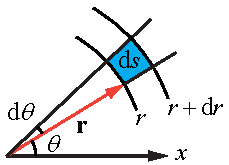
\includegraphics[width=4cm]{./figures/CrIntN1.pdf}
\caption{极坐标中的面积元} \label{CrIntN_fig1}
\end{figure}

我们来看如何在极坐标系中进行二重积分. 我们先把积分区域划分为无数个小面元, 点 $\vec r$ 处面元的形状如\autoref{CrIntN_fig1} 所示, 即把两个坐标 $r, \theta$ 坐标分别在原来的基础上增加一个微小值,并围成一块小区域. 由于 $\dd{r}, \dd{\theta}$ 都是无穷小, 该面元的形状趋近于长方形, 其面积为两边长相乘
\begin{equation}
\dd{s} = \dd{r}\cdot r\dd{\theta} = r\dd{r}\dd{\theta}
\end{equation}
类比\autoref{IntN_ex1}\upref{IntN}, 我们可以将 $f(r, \theta)$ 的面积分记为
\begin{equation}\label{CrInt_eq2}
\iint_{\mathcal S} f(r, \theta) r\dd{r}\dd{\theta} = \int_{\theta_1}^{\theta_2} \dd{\theta}\int_{r_1(\theta)}^{r_2(\theta)} \dd{r} r f(r, \theta)
\end{equation}
其中 $r_1(\theta)$ 与 $r_2(\theta)$ 是区域 $\mathcal S$ 的两条边界(类比\autoref{IntN_eq7} 中的 $y_1(x), y_2(x)$)

\begin{exam}{}
求 $f(r,\theta) = ar$ 在内外半径为 $R_1, R_2$ 的圆环区域的面积分. 

先来看积分上下限, 对于圆环区域, 显然有 $r_1(\theta) = R_1$, $r_2(\theta) = R_2$, $\theta_1 = 0$, $\theta_2 = 2\pi$. 直接使用\autoref{CrInt_eq2} 得
\begin{equation}\ali{
\iint_{\mathcal S} f(r, \theta) r\dd{r}\dd{\theta} &= \int_0^{2\pi} \qty[\int_{R_1}^{R_2} ar^2 \dd{r}] \dd{\theta}
= \int_0^{2\pi} \frac a3 (R_2^3 - R_1^3) \dd{\theta}\\
&= \frac{2\pi a}{3} (R_2^3 - R_1^3)
}\end{equation}

如果使用直角坐标系计算该积分, 过程将会变得十分复杂.
\end{exam}

% 未完成, 曲线坐标系应该在 柱坐标和球坐标的偏导 中完成
\subsection{曲线坐标系中的体积分}
我们接下来要讨论的曲线坐标系准确来说应该是\bb{正交曲线坐标系}, 假设三个坐标为 $x_1, x_2, x_3$, “正交” 指的是这种坐标系必须满足位置矢量对三个坐标的偏导数 $\pdv*{\vec r}{x_i} \,\, (i = 1,2,3)$ 必须两两垂直. 例如在柱坐标系中(位矢为 $\vec r = r\uvec r + z\uvec z$) 有
%未完成, 这个式子哪里冒出来的
\begin{equation}
\dd{\vec r} = \dd{r} \uvec r + r\dd{\theta} \uvec\theta + \dd{z}\uvec z
\end{equation}
三个偏微分分别为
\begin{equation}
\pdv{\vec r}{r} = \uvec r \qquad 
\pdv{\vec r}{\theta} = r \uvec \theta \qquad 
\pdv{\vec r}{z} = \uvec z
\end{equation}
满足两两垂直. 在球坐标系(位矢为 $\vec r = r\uvec r$)中有
\begin{equation}
\dd{\vec r} = \dd{r} \uvec r + r\dd{\theta} \uvec\theta + r\sin\theta\dd{\phi}\uvec\phi
\end{equation}
所以柱坐标和球坐标系的三个偏微分

可见三个偏导的方向就是三个单位矢量的方向,%未完成:矢量全微分和偏导的关系没讲.
满足两两垂直.

所以球坐标系和柱坐标系都是正交曲线坐标系. 另外我们熟知的直角坐标系也属于正交曲线坐标系. 以后我们会将“正交” 两字略去.

在曲线坐标系中, 令
\begin{equation}
\pdv{\vec r}{x_i} \equiv f_i(\vec r)\uvec x_i \quad (i = 1,2,3)
\end{equation}
则空间中的一个体积元(每个 $x_i$ 都分别增加 $\dd{x_i}$ 所围成的长方体)可以表示为
\begin{equation}
\dd{V} = f_1(\vec r)f_2(\vec r)f_3(\vec r)\dd{x_1}\dd{x_2}\dd{x_3}
\end{equation}
为了方便书写我们以后将 $\dd{x_1}\dd{x_2}\dd{x_3}$ 记为 $\dd[3]{x}$ 或 $\dd[3]{r}$.

\begin{figure}[ht]
\centering
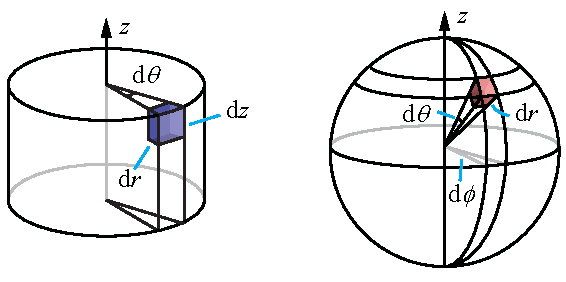
\includegraphics[width=9.5cm]{./figures/CrIntN2.pdf}
\caption{柱坐标(左)和球坐标(右)中的体积元} \label{CrIntN_fig2}
\end{figure}

我们已知直角坐标系中 $f_i(\vec r) = 1$, 体积元为 $\dd[3]{x}$. 现在我们还可以写出柱坐标系和球坐标系的体积元分别为
\begin{align}
\dd{V} &= r \dd{r}\dd{\theta}\dd{z}\\
\dd{V} &= r^2\sin\theta \dd{r}\dd{\theta}\dd{\phi}
\end{align}
柱坐标系和球坐标系中的体积元如\autoref{CrIntN_fig2} 所示